\chapter{Literatur}
	\section{Verwandte Arbeiten}
		In diesem Abschnitt wird auf vorhandene Arbeiten eingegangen, die sich mit der Problematik der Segmentierung von Bildern oder Punktwolken mit neuronalen Netzen befassen. 
		\subsection{PointNet}
			Das 2017 in \cite{PointNet} vorgestellte PointNet ist ein neuronales Netzwerk zum Auswerten von Punktwolken. Das Netz bietet dabei sowohl eine Architektur zur Klassifizierung als auch eine zur Segmentierung. Der Strukturelle Aufbau ist in Abbildung \ref{fig:pointnet} dargestellt. 
			\begin{figure}
				\centering
				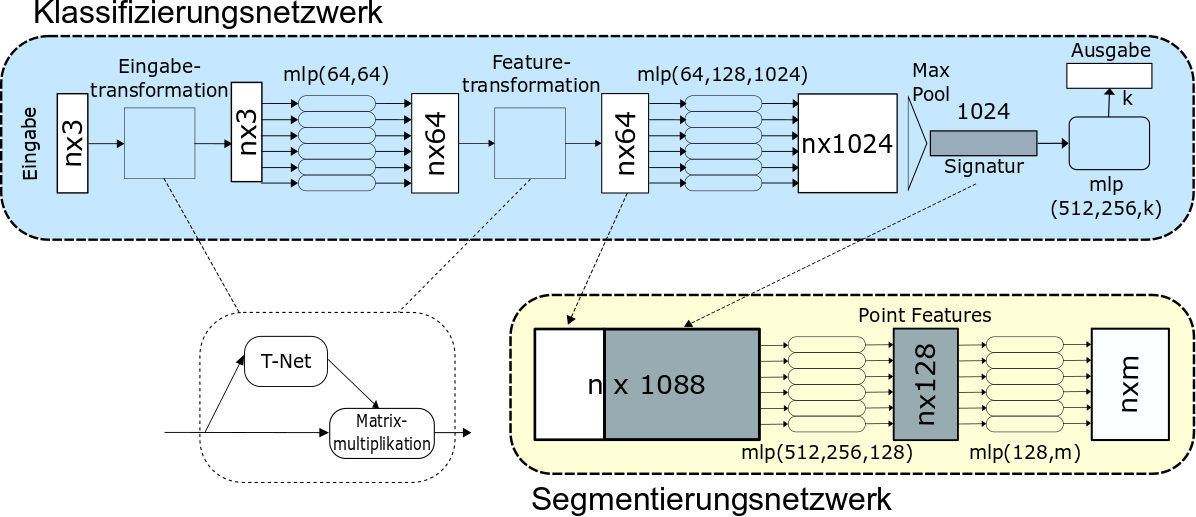
\includegraphics[width=15cm]{img/PointNet.png}
				\caption{Funktionsweise von PointNet}
				\label{fig:pointnet}
			\end{figure} 
			Problematisch an der Auswertung von Punktwolken mit Technologien der Neuroinformatik ist vor allem, dass die Daten im Allgemeinen ungeordnet sind. Das Netzwerk erzeugt darum aus einem Eingabevektor, der aus einer Menge von Koordinaten gebildet wird zun�chst durch Feature Transformation eine globale Signatur, also einen Feature-Vektor, der unabh�ngig von der Reihenfolge der Eingabegr��en ist. PointNet erreicht dies durch den Einstatz von Max-Pooling. Um Invarianz bez�glich bestimmter r�umlicher Transformationen wie z.B. Rotation zu erreichen, wird bei der Erstellung dieses globalen Feature-Vektor mit einem kleinen neuronalen Netz, dem "`T-Net"', eine Transformationsmatrix angen�hert und auf die Eingabedaten angewandt. Mit der so berechneten Signatur kann ein weiteres Netz, in diesem Fall ein MLP, trainiert werden, das diese klassifiziert. Da der globale Feature-Vektor keine Ortsinformationen enth�lt, ist es nicht m�glich, damit eine Segmentierung durchzuf�hren. Soll das Netzwerk also f�r diesen Zweck verwendet werden, wird der globale Feature-Vektor mit dem Eingabevektor kombiniert, um einen Vektor zu erzeugen, der sowohl globale als auch lokale Eigenschaften repr�sentiert. Anschlie�end kann ein Label f�r jeden Punkt gesch�tzt werden.
			
		\subsection{UPSNet}
			Das 2019 in \cite{UPSNet} vorgestellte UPSNet (Unified Panoptic Segmentation Network) ist ein neuronales Netz f�r panoptische Segmentierung. Dazu f�hrt das Netzwerk parallel eine semantische Segmentierung und eine Instanzsegmentierung des Eingabebildes durch und erstellte mit den kombinierten Ausgaben beider Methoden einen Tensor von Wahrscheinlichkeiten f�r jede Klasse und Instanz. Aus diesem Tensor wird in einem letzten Schritt ein Ausgabebild erzeugt. Der Aufbau des Netzwerks ist in Abbildung \ref{fig:upsarc} dargestellt.\\
			\begin{figure}
				\centering
				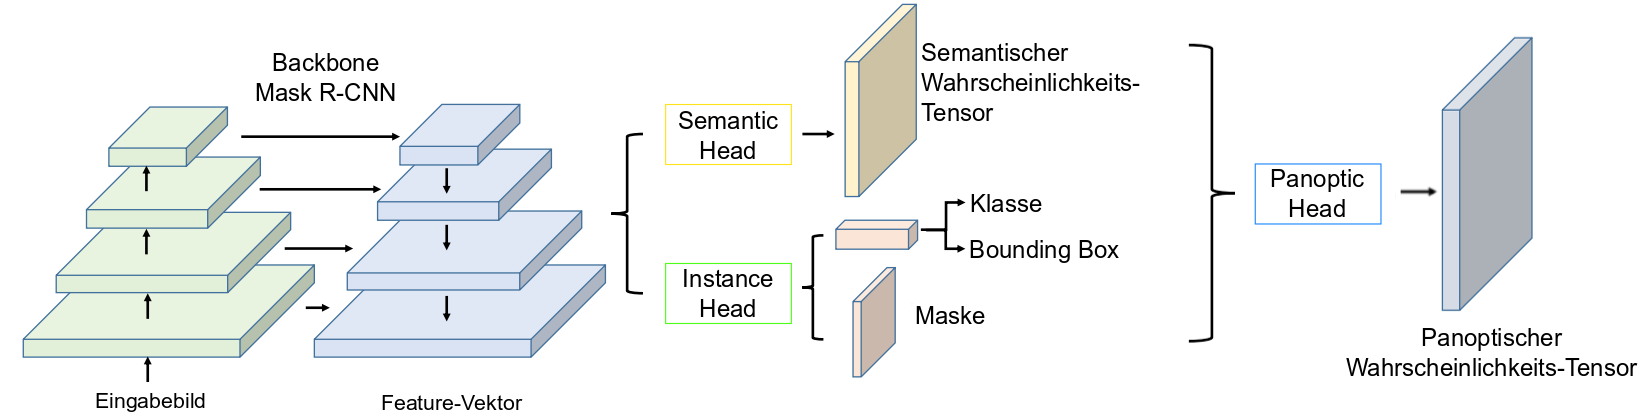
\includegraphics[width=15cm]{img/UPSNet.png}
				\caption{Architektur von UPSNet}
				\label{fig:upsarc}
			\end{figure} 
			UPSNet verwendet als Backbone das in \cite{MaskRCNN} beschriebene Mask R-CNN, das sich aus dem ResNet und dem Feature Pyramid Network \cite{FPN} ableitet. Mask R-CNN f�hrt eine Instanz-Segmentierung des Bildes durch und erzeugt parallel dazu eine Maske f�r jedes erkannte Objekt. Die Ausgabe des Backbones wird von zwei leichtgewichtigen Netzen, dem "`Semantic Segmentation Head"', der semantisch segmentiert und dem "`Instance Segmentation Head"', der eine Instanzsegmentierung durchf�hrt unabh�ngig voneinander weiterverarbeitet. Die Implementierung eines einzelnen Backbones spart Rechenzeit und Speicherplatz gegen�ber Architekturen mit zwei getrennten Netzen. Die daraus entstandenen Ergebnisse werden von dem "`Panoptic Segmentation Head"' anhand einer Heuristik ausgewertet, um die Netzwerkausgabe zu erstellen.\\
			Der "`Instance Segmentation Head"' folgt dem Konzept von Mask R-CNN und erzeugt eine Anzahl von Bounding Boxes und Masken. Der "`Semantic Segmentation Head"' ist ein CNN, das einen vom Backbone erzeugten Feature-Vektor als Eingabe erh�lt und mittels Soft-Max die Klasse jedes Pixels sch�tzt. Der "`Panoptic Segmentation Head"' ermittelt zuerst die Anzahl von im Bild vorhandener Instanzen und erstellt einen Tensor aus den von den beiden vorherigen K�pfen errechneten Wahrscheinlichkeiten und f�hrt eine Soft-Max Berechnung durch. Aus dem Resultat wird anhand einer Heuristik f�r jeden Pixel entschieden, ob er einer Instanz eines z�hlbaren Objekts und welcher Klasse er angeh�rt. Es ist dabei m�glich, dass Pixel als unbekannt klassifiziert werden, was den IoU der Ergebnisse durch die Verminderung von False Positives verbessert.